\color{black}
\subsection{Specifica componenti View::Component}
\label{specificaCompon}
\begin{figure}[!h]

			\includegraphics[width=\linewidth]{../Specifica_Tecnica/Content/Immagini/Romeo__View__Component.png}
			\caption{Componente Romeo::View::Component}
			\label{comp_romeo::view::component}
\end{figure}
\pagebreak
%%%%%%%%%%%%%%%%%%%
% 	TOOLBAR
%%%%%%%%%%%%%%%%%
\subsubsection{ToolBar(class)}
\label{spetool}
\begin{figure}[!h]
\centering
			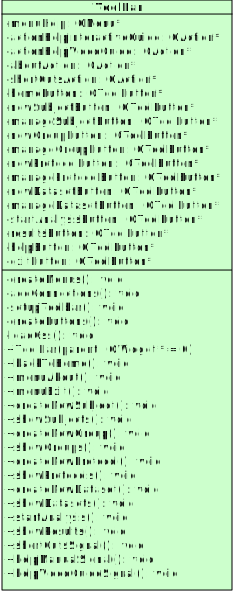
\includegraphics[width=0.4\linewidth]{./Content/Immagini/view/ToolBar.png}
			\caption{Diagramma Classe ToolBar: attributi e metodi}
			\label{cl_tool}
\end{figure}
\paragraph{Descrizione \\}
Classe che rappresenta la componente contenuta nelle finestre per poter filtrare i contenuti delle tabelle presentei nella vista in base a diversi parametri secondo le preferenze dell'utente.
\paragraph{Utilizzo\\}
La classe viene utilizzata per dare all'utente la possibilità di visualizzare i dati tabellari ordinandoli secondo una certa caratteristica scelta dall'utente nel momento in cui si trova sulla finestra che espone una tabella.
\paragraph{Classi ereditate\\}
\begin{itemize}
\item Qt::QWidget.
\end{itemize}
%%%%%%%%%%%%%% ATTRIBUTI
\paragraph{\textcolor{black}{Attributi\\}}
\begin{itemize}
%menuHelp
\item \color{teal}\verb!-menuHelp:QMenu*!
\color{black}
\subparagraph{Descrizione:} rappresenta il menu per l'help.
%actHelpInteractiveGuide
\item \color{teal}\verb! - actionHelpInteractiveGuide:QAction*!
\color{black} 
\subparagraph{Descrizione: } Rappresenta l'azione l'help interattivo.

%actHelpVideoGuide
\item \color{teal}\verb! - actionHelpVideoGuide:QAction*!
\color{black} 
\subparagraph{Descrizione: } Rappresenta l'azione per la video guida, elemento del menu help.

%aboutAct
\item \color{teal}\verb! - aboutAction:QAction*!
\color{black} 
\subparagraph{Descrizione: } Rappresenta l'azione per l'elemento about del menu help.

%shortCutHelp
\item \color{teal}\verb! - shortCutsAction:QAction*!
\color{black} 
\subparagraph{Descrizione: } Rappresenta l'azione per i shortcuts, elemento del menu help.
%%%%%%%%%%%%%%%%% qtoolbutton
\item \color{teal}\verb!-homeButton: QToolButton*!
\color{black}
\subparagraph{Descrizione:} Rappresenta il pulsante della toolbar per raggiungere la pagina iniziale dell'applicativo \project{}.

\item \color{teal}\verb!-newSubjectButton: QToolButton*!
\color{black}
\subparagraph{Descrizione:} Rappresenta il pulsante della toolbar per raggiungere la view per la creazione di un nuovo Subject\g{} dell'applicativo \project{}.

\item \color{teal}\verb!-newGroupButton: QToolButton*!
\color{black}
\subparagraph{Descrizione:} Rappresenta il pulsante della toolbar per raggiungere la view per la creazione di un nuovo gruppo di Subject\g{} dell'applicativo \project{}.

\item \color{teal}\verb!-newProtocolButton: QToolButton*!
\color{black}
\subparagraph{Descrizione:} Rappresenta il pulsante della toolbar per raggiungere la view per la creazione di un nuovo Protocol\g{} dell'applicativo \project{}.

\item \color{teal}\verb!-newDatasetButton: QToolButton*!
\color{black}
\subparagraph{Descrizione:} Rappresenta il pulsante della toolbar per raggiungere la view per la creazione di un nuovo Dataset\g{} dell'applicativo \project{}.

\item \color{teal}\verb!-manageSubjectButton: QToolButton*!
\color{black}
\subparagraph{Descrizione:} Rappresenta il pulsante della toolbar per raggiungere la view per la gestione dei Subject\g{} dell'applicativo \project{}.

\item \color{teal}\verb!-manageGroupButton: QToolButton*!
\color{black}
\subparagraph{Descrizione:} Rappresenta il pulsante della toolbar per raggiungere la view per la gestione dei gruppi di Subject\g{} dell'applicativo \project{}.

\item \color{teal}\verb!-manageProtocolButton: QToolButton*!
\color{black}
\subparagraph{Descrizione:} Rappresenta il pulsante della toolbar per raggiungere la view per la gestione dei Protocol\g{} dell'applicativo \project{}.

\item \color{teal}\verb!-manageDatasetButton: QToolButton*!
\color{black}
\subparagraph{Descrizione:} Rappresenta il pulsante della toolbar per raggiungere la view per la gestione dei Dataset\g{} dell'applicativo \project{}.

\item \color{teal}\verb!-startAnalysisButton: QToolButton*!
\color{black}
\subparagraph{Descrizione:} Rappresenta il pulsante della toolbar per raggiungere la view per creare e avviare una nuova analisi dell'applicativo \project{}.

\item \color{teal}\verb!-resultsButton: QToolButton*!
\color{black}
\subparagraph{Descrizione:} Rappresenta il pulsante della toolbar per raggiungere la view per la visualizzazione dei risultati delle analisi effettuate dell'applicativo \project{}.

\item \color{teal}\verb!-helpButton: QToolButton*!
\color{black}
\subparagraph{Descrizione:} Rappresenta il pulsante della toolbar per ottenere maggiori aiuti nell'utilizzo dell'applicativo \project{}.

\item \color{teal}\verb!-exitButton: QToolButton*!
\color{black}
\subparagraph{Descrizione:} Rappresenta il pulsante della toolbar per chiudere l'applicativo \project{}.
\end{itemize}

%%%%%%%%%%%%%%%%%%%%%%

%%%%%%%%%  METODI
\paragraph{\textcolor{black}{Metodi\\}}
\begin{itemize}
%costruttore
\item \color{blue}\verb! + ToolBar(parent : QWidget*=0)!
\color{black}
\subparagraph{Descrizione:}
Costruttore per la classe ToolBar. \\
\subparagraph{Argomenti}
\begin{itemize}
\item \color{RoyalPurple} \verb!parent: QWidget*=0 ! \\ Puntatore al QWidget padre di ToolBar.
\end{itemize}

%setupToolBar()
\item \color{blue}\verb! -setupToolBar():void!
\color{black}
\subparagraph{Descrizione:} Metodo che ha il compito di impostare le configurazioni del menu e creare i componenti della la toolbar.
\color{black}
%createMenus()
\item \color{blue}\verb! -createMenus():void!
\color{black}
\subparagraph{Descrizione:} Metodo che ha il compito creare il menu di help.

%addConnection
\item \color{blue}\verb! -addConnections():void!
\color{black}
\subparagraph{Descrizione:} Metodo che ha il compito di impostare le connessioni tra i pulsanti e i Signal\g{}.

%createButtons
\item \color{blue}\verb! -createButtons():void!
\color{black}
\subparagraph{Descrizione:} Metodo che ha il compito di creare i pulsanti per la toolbar.

%css()
\item \color{blue}\verb! -loadCss():void!
\color{black}
\subparagraph{Descrizione:} Metodo che ha il compito di impostare lo stile per la toolbar.
%%%%%%%% signals
%backtohome
\item \color{blue}\verb! +backToHome():void! (signal)
\color{black} 
\subparagraph{Descrizione:} Signal\g{} emesso quando viene premuto il pulsante home dalla toolbar.

%menuAbo
\item \color{blue}\verb! +menuAbout():void! (signal)
\color{black} 
\subparagraph{Descrizione:} Signal\g{} emesso quando viene premuta l'azione \textit{about}.

%menuExit
\item \color{blue}\verb! +menuExit():void! (signal)
\color{black} 
\subparagraph{Descrizione:} Signal\g{} emesso quando viene premuto il pulsante exit dalla toolbar.

%createNewSub
\item \color{blue}\verb! +createNewSubject():void! (signal)
\color{black} 
\subparagraph{Descrizione:} Signal\g{} emesso quando viene premuto il pulsante per la creazione di un nuovo Subject\g{} dalla toolbar.

%createNewGrou
\item \color{blue}\verb! +createNewGroup():void! (signal)
\color{black} 
\subparagraph{Descrizione:} Signal\g{} emesso quando viene premuto il pulsante per la creazione di un nuovo gruppo di Subject\g{} dalla toolbar.

%createNewProt
\item \color{blue}\verb! +createNewProtocol():void! (signal)
\color{black} 
\subparagraph{Descrizione:} Signal\g{} emesso quando viene premuto il pulsante per la creazione di un nuovo Protocol\g{} dalla toolbar.

%createNewDAtaset
\item \color{blue}\verb! +createNewDataset():void! (signal)
\color{black} 
\subparagraph{Descrizione:} Signal\g{} emesso quando viene premuto il pulsante per la creazione di un nuovo Dataset\g{} dalla toolbar.


%showSub
\item \color{blue}\verb! +showSubjects():void! (signal)
\color{black} 
\subparagraph{Descrizione:} Signal\g{} emesso quando viene premuto il pulsante per la gestione dei Subject\g{} dalla toolbar.

%showGrou
\item \color{blue}\verb! +showGroups():void! (signal)
\color{black} 
\subparagraph{Descrizione:} Signal\g{} emesso quando viene premuto il pulsante per la gestione dei gruppi di Subject\g{} dalla toolbar.

%showprot
\item \color{blue}\verb! +showProtocols():void! (signal)
\color{black} 
\subparagraph{Descrizione:} Signal\g{} emesso quando viene premuto il pulsante per la gestione dei Protocol\g{} dalla toolbar.
%showDatas
\item \color{blue}\verb! +showDatasets():void! (signal)
\color{black} 
\subparagraph{Descrizione:} Signal\g{} emesso quando viene premuto il pulsante per la gestione dei Dataset\g{} dalla toolbar.

%showResult
\item \color{blue}\verb! +showResults():void! (signal)
\color{black} 
\subparagraph{Descrizione:} Signal\g{} emesso quando viene premuto il pulsante per la visualizzazione dei risultati dalla toolbar.

%startAnal
\item \color{blue}\verb! +startAnalysis():void! (signal)
\color{black} 
\subparagraph{Descrizione:} Signal\g{} emesso quando viene premuto il pulsante per la creazione e l'avvio di un'analisi dalla toolbar.

%shortcuts
\item \color{blue}\verb! +shortCutsSignal():void! (signal)
\color{black} 
\subparagraph{Descrizione:} Signal\g{} emesso quando viene premuto il pulsante per la visualizzazione degli shortcut disponibili dalla toolbar.

%helpManual
\item \color{blue}\verb! +helpManualSignal():void! (signal)
\color{black} 
\subparagraph{Descrizione:} Signal\g{} emesso quando viene premuta l'azione per la visualizzazione del manuale di utilizzo dalla toolbar.

%video
\item \color{blue}\verb! +helpVideoGuideSignal():void! (signal)
\color{black} 
\subparagraph{Descrizione:} Signal\g{} emesso quando viene premuta l'azione per la visualizzazione della video guida.
\end{itemize}
\pagebreak
\color{black}


%%%%%%%%%%%%%%%%%%
%	SELECTDESELECT
%%%%%%%%%%%%%%%%%%
\subsubsection{SelectDeselectWidget (class)}
\label{speselDes}
\begin{figure}[!h]
\centering
			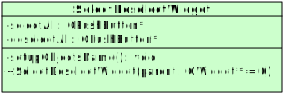
\includegraphics[width=0.5\linewidth]{./Content/Immagini/view/SelectDeselectWidget.png}
			\caption{Diagramma Classe SelectDeselectWidget: attributi e metodi}
			\label{cl_seldesel}
\end{figure}
\paragraph{Descrizione \\}
Classe che rappresenta la componente che permette, dove previsto, di velocizzare le operazioni dell'utente qualora voglia selezionare (o deselezionare) l'intero insieme dei dati.
\paragraph{Utilizzo\\}
La classe viene utilizzata dalle viste che presentano un elenco di dati, che l'utente può selezionare per poi compiere determinate azioni sugli elementi scelti. È molto utile quando l'utente ha da selezionare (rispettivamente, deselezionare) un numero molto alto di voci.
\paragraph{Classi ereditate\\}
\begin{itemize}
\item Qt::QWidget.
\end{itemize}
%%%%%%%%%%%%%%ATTRIBUTI%%%%%%%%%%%
\paragraph{\textcolor{black}{Attributi\\}}
\begin{itemize}
\item \color{teal}\verb!-selectAll: QPushButton*!
\color{black}
\subparagraph{Descrizione:} Pulsante che permette la selezione contemporanea di tutte le voci della tabella.

\item \color{teal}\verb!-deselectAll: QPushButton*!
\color{black}
\subparagraph{Descrizione:} Pulsante che permette la deselezione contemporanea di tutte le voci della tabella.
\end{itemize}
%%%%%%%%%  METODI
\paragraph{\textcolor{black}{Metodi\\}}
\begin{itemize}
%costruttore
\item \color{blue}\verb! + SelectDeselectWidget(parent : QWidget*=0)!
\color{black}
\subparagraph{Descrizione:} Costruttore per la classe SelectDeselectWidget.
\subparagraph{Argomenti:}
\begin{itemize}
\item \color{RoyalPurple} \verb!parent: QWidget*=0 ! \\ Puntatore al QWidget padre di ToolBar.
\end{itemize}

%setupObjName()
\item \color{blue}\verb! -setupObjectName():void!
\color{black}
\subparagraph{Descrizione:} Metodo che ha il compito di impostare i nomi degli oggetti contenuti all'interno del widget \emph{SelectDeselectAll}.
\end{itemize}
\color{black}
\pagebreak


%%%%%%%%%%%%%%%%
%	NAVWIDGET
%%%%%%%%%%%%%%%%
\subsubsection{NavWidget (class)}
\label{spenav}
\begin{figure}[!h]
\centering
			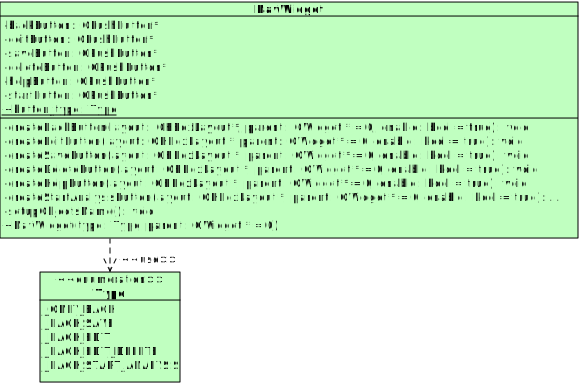
\includegraphics[width=0.9\linewidth]{./Content/Immagini/view/NavWidget.png}
			\caption{Diagramma Classe NavWidget: attributi e metodi}
			\label{cl_nav}
\end{figure}
\paragraph{Descrizione \\}
Classe che rappresenta la componente disposta nella parte bassa del layout della finestra contenente i pulsanti per la navigazione all'indietro, la visualizzazione della guida interattiva e, ove previsti, i pulsanti per la modifica, per la cancellazione e per il salvataggio delle modifiche apportate.
\paragraph{Utilizzo\\}
La classe viene utilizzata da tutte le viste in quanto è sicuramente sempre presente il pulsante per ritornare alla finestra precedente e per l'apertura della guida; gli altri pulsanti saranno presenti ove vi è la possibilità di effettuare operazioni che influiscono sullo stato del sistema come per esempio l'inserimento di un nuovo \subject{} o la cancellazione di un \protocol{} o ancora la modifica di un gruppo di \subject{}.
\paragraph{Classi ereditate\\}
\begin{itemize}
\item Qt::QWidget.
\end{itemize}
%%%%%%%%%%%%%%ATTRIBUTI%%%%%%%%%%%
\paragraph{\textcolor{black}{Attributi\\}}
\begin{itemize}
\item \color{teal}\verb!-backButton: QPushButton*!
\color{black}
\subparagraph{Descrizione: }Pulsante che permette il ritorno alla finestra precedente.

\item \color{teal}\verb!-editButton: QPushButton*!
\color{black}
\subparagraph{Descrizione: }Pulsante che permette la modifica di alcuni dati visualizzati nella vista.

\item \color{teal}\verb!-saveButton: QPushButton*!
\color{black}
\subparagraph{Descrizione: }Pulsante che permette il salvataggio delle modifiche precedentemente effettuate.

\item \color{teal}\verb!-deleteButton: QPushButton*!
\color{black}
\subparagraph{Descrizione: }Pulsante che permette la rimozione degli oggetti selezionati.

\item \color{teal}\verb!-helpButton: QPushButton*!
\color{black}
\subparagraph{Descrizione: }Pulsante che permette la visualizzazione della guida interattiva.

\item \color{teal}\verb!-startButton: QPushButton*!
\color{black}
\subparagraph{Descrizione: }Pulsante che permette di avviare una nuova analisi.

\item \color{teal}\verb!-restartButton: QPushButton*!
\color{black}
\subparagraph{Descrizione: }Pulsante che permette di riavviare un'analisi.

\item \color{teal}\verb!-showButton: QPushButton*!
\color{black}
\subparagraph{Descrizione: }Pulsante che permette visualizzare i risultati delle analisi.
\end{itemize}
%%%%%%%%%  METODI
\paragraph{\textcolor{black}{Metodi\\}}
\begin{itemize}
%costruttore
\item \color{blue}\verb! + NavWidget(type: Type, parent : QWidget*=0)!
\color{black}
\subparagraph{Descrizione: }
Costruttore per la classe NavWidget. 
\subparagraph{Argomenti:}
\begin{itemize}
\item \color{RoyalPurple} \verb! type: Type !\\ suggerisce la tipologia di NavWidget da costruire:
\begin{itemize}
\item solo ritorno alla finestra precedente e visualizzazione guida (es. visualizzazione \subject{} presenti nel sistema);
\item ritorno alla finestra precedente e salvataggio operazioni (es. per le viste che si occupano di creare nuovi elementi);
\item ritorno alla finestra precedente e possibilità di modifica dei campi (es. visualizzazione gruppi di \subject{});
\item ritorno alla finestra precedente e possibilità di cancellare elementi selezionati (es. visualizzazione \protocol{});
\item ritorno alla finestra precedente e possibilità di avviare l'analisi (es. starAnalysis);
\item ritorno alla finestra precedente e possibilità di riavviare l'analisi e visualizzare i risultati.
\end{itemize}
\item  \color{RoyalPurple} \verb! parent: QWidget*=0 ! \\ Puntatore al QWidget padre di ToolBar.
\end{itemize}

%setupObjName()
\item \color{blue}\verb!-setupObjectName():void!
\color{black}
\subparagraph{Descrizione:} Metodo che ha il compito di impostare i nomi degli oggetti contenuti all'interno del widget \emph{SelectDeselectAll}.

\color{black}
%createBackButton
\item \color{blue}\verb!-createBackButton(layout:QHBoxLayout*, parent:QWidget*= 0, enable:bool= true): void!
\color{black}
\subparagraph{Descrizione: }Metodo che ha il compito di creare il campo dati \emph{backButton}.
\subparagraph{Argomenti:}
\begin{itemize}
\item \color{RoyalPurple} \verb! layout: QHBoxLayout*! \\ box per dare un'allineamento orizzontale del pulsante;
\item  \color{RoyalPurple} \verb!parent: QWidget*=0 ! \\ Puntatore al QWidget padre di NavWidget;
\item  \color{RoyalPurple} \verb!enable: bool=true! \\ caratteristica del pulsante ad essere abilitato alla pressione, di default è true.
\end{itemize}

%createEditButton
\item \color{blue}\verb!-createEditButton(layout:QHBoxLayout*, parent:QWidget*=0, enable:bool=true):void!
\color{black}
\subparagraph{Descrizione: }Metodo che ha il compito di creare il campo dati \emph{editButton}.
\subparagraph{Argomenti: }
\begin{itemize}
\item  \color{RoyalPurple} \verb!layout: QHBoxLayout* !\\ box per dare un'allineamento orizzontale del pulsante;
\item  \color{RoyalPurple} \verb!parent: QWidget*=0!  \\ Puntatore al QWidget padre di NavWidget;
\item  \color{RoyalPurple} \verb!enable: bool=true !\\ caratteristica del pulsante ad essere abilitato alla pressione, di default è true.
\end{itemize}

%createSaveButton
\item \color{blue}\verb!-createSaveButton(layout:QHBoxLayout*, parent:QWidget*=0, enable:bool= true):void!
\color{black}
\subparagraph{Descrizione: }Metodo che ha il compito di creare il campo dati \emph{saveButton}.
\subparagraph{Argomenti:}
\begin{itemize}
\item  \color{RoyalPurple} \verb!layout: QHBoxLayout* !\\ box per dare un'allineamento orizzontale del pulsante;
\item  \color{RoyalPurple} \verb!parent: QWidget*=0 ! \\ Puntatore al QWidget padre di NavWidget;
\item  \color{RoyalPurple} \verb!enable: bool=true !\\ caratteristica del pulsante ad essere abilitato alla pressione, di default è true.
\end{itemize}

%createdeleteButton
\item \color{blue}\verb!-createDeleteButton(layout:QHBoxLayout*, parent:QWidget*=0, enable:bool=true):void!
\color{black}
\subparagraph{Descrizione: } Metodo che ha il compito di creare il campo dati \emph{deleteButton}.
\subparagraph{Argomenti:}
\begin{itemize}
\item \color{RoyalPurple} \verb! layout: QHBoxLayout*! \\ box per dare un'allineamento orizzontale del pulsante;
\item  \color{RoyalPurple} \verb!parent: QWidget*=0 ! \\ Puntatore al QWidget padre di NavWidget;
\item  \color{RoyalPurple} \verb!enable: bool=true! \\ caratteristica del pulsante ad essere abilitato alla pressione, di default è true.
\end{itemize}
%createHelpButton
\item \color{blue}\verb!-createHelpButton(layout:QHBoxLayout*, parent:QWidget*=0, enable:bool=true):void!
\color{black}
\subparagraph{Descrizione:} Metodo che ha il compito di creare il campo dati \emph{helpButton}.
\subparagraph{Argomenti:}
\begin{itemize}
\item  \color{RoyalPurple} \verb!layout: QHBoxLayout*! \\ box per dare un'allineamento orizzontale del pulsante;
\item  \color{RoyalPurple} \verb!parent: QWidget*=0  !\\ Puntatore al QWidget padre di NavWidget;
\item  \color{RoyalPurple} \verb!enable: bool=true !\\ caratteristica del pulsante ad essere abilitato alla pressione, di default è true.
\end{itemize}

%createStartButton
\item \color{blue}\verb!-createStartAnalysisButton(layout:QHBoxLayout*, parent:QWidget*=0, enable:bool=true):void!
\color{black}
\subparagraph{Descrizione:} Metodo che ha il compito di creare il campo dati \emph{startButton}.
\subparagraph{Argomenti:}
\begin{itemize}
\item  \color{RoyalPurple} \verb!layout: QHBoxLayout*! \\ box per dare un'allineamento orizzontale del pulsante;
\item  \color{RoyalPurple} \verb!parent: QWidget*=0 ! \\ Puntatore al QWidget padre di NavWidget;
\item  \color{RoyalPurple} \verb!enable: bool=true !\\ caratteristica del pulsante ad essere abilitato alla pressione, di default è true.
\end{itemize}

%createSshowButton
\item \color{blue}\verb!-createShowButton(layout:QHBoxLayout*, parent:QWidget*=0, enable:bool=true):void!
\color{black}
\subparagraph{Descrizione:} Metodo che ha il compito di creare il campo dati \emph{showButton}.
\subparagraph{Argomenti:}
\begin{itemize}
\item  \color{RoyalPurple} \verb!layout: QHBoxLayout*! \\ box per dare un'allineamento orizzontale del pulsante;
\item  \color{RoyalPurple} \verb!parent: QWidget*=0 ! \\ Puntatore al QWidget padre di NavWidget;
\item  \color{RoyalPurple} \verb!enable: bool=true !\\ caratteristica del pulsante ad essere abilitato alla pressione, di default è true.
\end{itemize}

%createrestartButton
\item \color{blue}\verb!-createRestartButton(layout:QHBoxLayout*, parent:QWidget*=0, enable:bool=true):void!
\color{black}
\subparagraph{Descrizione:} Metodo che ha il compito di creare il campo dati \emph{restartButton}.
\subparagraph{Argomenti:}
\begin{itemize}
\item  \color{RoyalPurple} \verb!layout: QHBoxLayout*! \\ box per dare un'allineamento orizzontale del pulsante;
\item  \color{RoyalPurple} \verb!parent: QWidget*=0 ! \\ Puntatore al QWidget padre di NavWidget;
\item  \color{RoyalPurple} \verb!enable: bool=true !\\ caratteristica del pulsante ad essere abilitato alla pressione, di default è true.
\end{itemize}

%%%%%%%%%%%%%%%%%%%%%%% setEnable
%setEnableBack
\item \color{blue}\verb!+setEnableBack(enable:bool=true):void!
\color{black}
\subparagraph{Descrizione:} Metodo che ha il compito di impostare la proprietà \textit{enable:} del pulsante \textit{back}.
\subparagraph{Argomenti:}
\begin{itemize}
\item  \color{RoyalPurple} \verb!enable: bool=true !\\ caratteristica del pulsante ad essere abilitato alla pressione, di default è true.
\end{itemize}

%setEnableedit
\item \color{blue}\verb!+setEnableEdit(enable:bool=true):void!
\color{black}
\subparagraph{Descrizione:} Metodo che ha il compito di impostare la proprietà \textit{enable:} del pulsante \textit{edit}.
\subparagraph{Argomenti:}
\begin{itemize}
\item  \color{RoyalPurple} \verb!enable: bool=true !\\ caratteristica del pulsante ad essere abilitato alla pressione, di default è true.
\end{itemize}

%setEnablesave
\item \color{blue}\verb!+setEnableSave(enable:bool=true):void!
\color{black}
\subparagraph{Descrizione:} Metodo che ha il compito di impostare la proprietà \textit{enable:} del pulsante \textit{save}.
\subparagraph{Argomenti:}
\begin{itemize}
\item  \color{RoyalPurple} \verb!enable: bool=true !\\ caratteristica del pulsante ad essere abilitato alla pressione, di default è true.
\end{itemize}

%setEnableDelete
\item \color{blue}\verb!+setEnableDelete(enable:bool=true):void!
\color{black}
\subparagraph{Descrizione:} Metodo che ha il compito di impostare la proprietà \textit{enable:} del pulsante \textit{delete}.
\subparagraph{Argomenti:}
\begin{itemize}
\item  \color{RoyalPurple} \verb!enable: bool=true !\\ caratteristica del pulsante ad essere abilitato alla pressione, di default è true.
\end{itemize}

%setEnableStart
\item \color{blue}\verb!+setEnableStartAnalyis(enable:bool=true):void!
\color{black}
\subparagraph{Descrizione:} Metodo che ha il compito di impostare la proprietà \textit{enable:} del pulsante \textit{startAnalysis}.
\subparagraph{Argomenti:}
\begin{itemize}
\item  \color{RoyalPurple} \verb!enable: bool=true !\\ caratteristica del pulsante ad essere abilitato alla pressione, di default è true.
\end{itemize}

%setEnablerestart
\item \color{blue}\verb!+setEnableRestart(enable:bool=true):void!
\color{black}
\subparagraph{Descrizione:} Metodo che ha il compito di impostare la proprietà \textit{enable:} del pulsante \textit{restart}.
\subparagraph{Argomenti:}
\begin{itemize}
\item  \color{RoyalPurple} \verb!enable: bool=true !\\ caratteristica del pulsante ad essere abilitato alla pressione, di default è true.
\end{itemize}

%setEnableshow
\item \color{blue}\verb!+setEnableShow(enable:bool=true):void!
\color{black}
\subparagraph{Descrizione:} Metodo che ha il compito di impostare la proprietà \textit{enable:} del pulsante \textit{show}.
\subparagraph{Argomenti:}
\begin{itemize}
\item  \color{RoyalPurple} \verb!enable: bool=true !\\ caratteristica del pulsante ad essere abilitato alla pressione, di default è true.
\end{itemize}

%setEnablehelp
\item \color{blue}\verb!+setEnableHelp(enable:bool=true):void!
\color{black}
\subparagraph{Descrizione:} Metodo che ha il compito di impostare la proprietà \textit{enable:} del pulsante \textit{help}.
\subparagraph{Argomenti:}
\begin{itemize}
\item  \color{RoyalPurple} \verb!enable: bool=true !\\ caratteristica del pulsante ad essere abilitato alla pressione, di default è true.
\end{itemize}

%create
\item \color{blue}\verb! -create(type: Type, navContainerLayout: QHBoxLayout, helpContainerLayout: QHBoxLayout)!
\color{black}
Costruttore per la classe NavWidget. \\
\subparagraph{Argomenti:}
\begin{itemize}
\item \color{RoyalPurple} \verb! type: Type !\\ Rappresenta quali pulsanti verranno visualizzati nel widget;
\item \color{RoyalPurple} \verb! navContainerLayout: QHBoxLayout* !\\ Rappresenta il layout per i pulsanti di navigazione;
\item \color{RoyalPurple} \verb! helpContainerLayout: QHBoxLayout* !\\ Rappresenta il layout per il pulsante di help.
\end{itemize}

\end{itemize}
\color{black}
\pagebreak

%%%%%%%%%%%%%%%%%%%%%%%%%%%%%%
% 	IMAGELABEL
%%%%%%%%%%%%%%%%%%%%%%%%%
\subsubsection{ImageLabel (class)}
\label{speImage}
\begin{figure}[!h]
\centering
			\includegraphics[width=0.6\linewidth]{./Content/Immagini/view/ImageLabel.png}
			\caption{Diagramma Classe ImageLabel: attributi e metodi}
			\label{cl_image}
\end{figure}
\paragraph{Descrizione \\}
Classe che rappresenta l'immagine di un Subject\g{} o dell'analisi alla con la quale si può interagire facendo doppio click.
\paragraph{Utilizzo\\}
La classe viene utilizzata dalle classi SubjectsView e  detailedResultsView per visualizzare le anteprime delle immagini con le quali l'utente può interagire.
\paragraph{Classi ereditate\\}
\begin{itemize}
\item Qt::QLabel.
\end{itemize}
%%%%%%%%%%%%%%ATTRIBUTI%%%%%%%%%%%
\paragraph{\textcolor{black}{Attributi\\}}
\begin{itemize}
\item \color{teal}\verb!-path: QString!
\color{black}
\subparagraph{Descrizione:} Rappresenta il path dell'immagine.
\end{itemize}
%%%%%%%%%% METODI %%%%%%%%%%%%%

\paragraph{\textcolor{black}{Metodi\\}}
\begin{itemize}
%costruttore
\item \color{blue}\verb! + ImageLabel(pathP: const QString&, parent : QWidget*=0)!
\color{black}
\subparagraph{Descrizione: }
Costruttore per la classe ImageLabel.
\subparagraph{Argomenti:}
\begin{itemize}
\item \color{RoyalPurple} \verb! pathP: const QString& ! \\ Rappresenta il path relativo all'immagine.
\item  \color{RoyalPurple} \verb! parent: QWidget*=0 ! \\ Puntatore al QWidget padre di ImageLabel.
\end{itemize}

%mouseDoubleclick
\item \color{blue}\verb! # mouseDoubleClickEvent(event:QMouseEvent*):void!
\color{black}
\paragraph{Descrizione:} Metodo virtuale della classe QLabel ridefinito per il doppio click del mouse.
\subparagraph{Argomenti:}
\begin{itemize}
\item \color{RoyalPurple} \verb! event: QMouseEvent*! \\ Rappresenta l'evento di pressione del mouse.
\end{itemize}

%setImage
\item \color{blue}\verb! + setImage(image:QImage &, dimension:int):void!
\color{black}
\paragraph{Descrizione:} Metodo che ha il compito di impostare l'immagine nella label con la dimensione passata come parametro
\subparagraph{Argomenti:}
\begin{itemize}
\item \color{RoyalPurple} \verb! image: QImage& ! \\ Rappresenta l'immagine da ridimensionare;
\item \color{RoyalPurple} \verb! dimension: int! \\ Rappresenta la dimensione a cui scalare l'immagine.
\end{itemize}

%signaldoubleclicked
\item \color{blue}\verb! + signalDoubleClicked(path:const QString &) :void!
\color{black}
\paragraph{Descrizione:} Signal\g{} emesso quando sulla lable viene fatto il doppio click con il mouse.
\subparagraph{Argomenti:}
\begin{itemize}
\item \color{RoyalPurple} \verb! path: const QString& ! \\ Rappresenta il path dell'immagine contenuta nella label;
\end{itemize}

\end{itemize}
\color{black}
\pagebreak
%%%%%%%%%%%%%%%%%%%%%%%%%%%%%%
% 	RESULTMESSAGEWIDGET
%%%%%%%%%%%%%%%%%%%%%%%%%
\subsubsection{ResultMessageWidget (class)}
\label{speResult}
\begin{figure}[!h]
\centering
			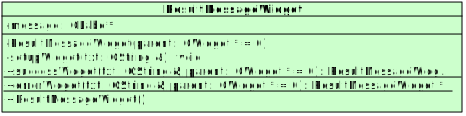
\includegraphics[width=0.7\linewidth]{./Content/Immagini/view/ResultMessageWidget.png}
			\caption{Diagramma Classe ResultMessageWidget: attributi e metodi}
			\label{cl_resMess}
\end{figure}
\paragraph{Descrizione \\}
Classe che rappresenta il widget che visualizza i messaggi dopo aver fatto un azione di salvataggio, modifica o eliminazione.
Il messaggio può essere di successo o di errore.
\paragraph{Utilizzo\\}
La classe viene utilizzata dalle varie viste per segnalare all'utente il successo o errore di un'azione fatta.
\paragraph{Classi ereditate\\}
\begin{itemize}
\item Qt::QWidget.
\end{itemize}
%%%%%%%%%%%%%%ATTRIBUTI%%%%%%%%%%%
\paragraph{\textcolor{black}{Attributi\\}}
\begin{itemize}
\item \color{teal}\verb!-message: QLabel*!
\color{black}
\subparagraph{Descrizione:} Rappresenta la label per il messaggio di testo da visualizzare.
\end{itemize}
%%%%%%%%%% METODI %%%%%%%%%%%%%
\paragraph{\textcolor{black}{Metodi\\}}
\begin{itemize}
%costruttore
\item \color{blue}\verb! -ResultMessageWidget(parent : QWidget*=0)!
\color{black}
\subparagraph{Descrizione: }
Costruttore per la classe ResultMessageWidget.
\subparagraph{Argomenti:}
\begin{itemize}
\item  \color{RoyalPurple} \verb! parent: QWidget*=0 ! \\ Puntatore al QWidget padre di ResultMessageWidget.
\end{itemize}
%setupWidget
\item \color{blue}\verb! -setupWidget(txt: const QString&):void!
\color{black}
\paragraph{Descrizione: }Metodo che ha il compito di impostare il componente e il layout del widget
\subparagraph{Argomenti:}
\begin{itemize}
\item \color{RoyalPurple} \verb! txt: const QString& ! \\ Rappresenta il testo da visualizzare.
\end{itemize}
%successWidget
\item \color{blue}\verb! -successWidget(txt: const QString&,parent: QWidget*=0):ResultMessageWidget*!
\color{black}
\paragraph{Descrizione: }Metodo che ha il compito di creare un ResultMessageWidget di successo. Ritorna il puntatore al widget creato.
\subparagraph{Argomenti:}
\begin{itemize}
\item \color{RoyalPurple} \verb! txt: const QString& ! \\ Rappresenta il testo da visualizzare nel widget;
\item  \color{RoyalPurple} \verb! parent: QWidget*=0 ! \\ Puntatore al QWidget padre di ResultMessageWidget.
\end{itemize}
\subparagraph{Note:}
\begin{itemize}
\item il metodo deve essere marcato statico.
\end{itemize}

%errorWidget
\item \color{blue}\verb! -errorWidget(txt: const QString&,parent: QWidget*=0):ResultMessageWidget*!
\color{black}
\paragraph{Descrizione: }Metodo che ha il compito di creare un ResultMessageWidget di errore. Ritorna il puntatore al widget creato.
\subparagraph{Argomenti:}
\begin{itemize}
\item \color{RoyalPurple} \verb! txt: const QString& ! \\ Rappresenta il testo da visualizzare nel widget;
\item  \color{RoyalPurple} \verb! parent: QWidget*=0 ! \\ Puntatore al QWidget padre di ResultMessageWidget.
\end{itemize}
\subparagraph{Note:}
\begin{itemize}
\item il metodo deve essere marcato statico.
\end{itemize}

\end{itemize}


